\chapter{Simulation}


\section{Randbedingungen}

Die Regelung benötigt eine Erkennung des aktuellen Phasenwinkelabschnitts, diese ist implementiert nach \cite{InstituteofElectricalandElectronicsEngineers}.

\section{IAF}

\cite{IAF99}

\subsection{Auslegung der Induktivitäten }
\subsection{Regelung}

\subsection{Ergebnisse}


\section{B6 1/3 PFC Buck}
Die in Kapitel \ref{sec:GrundlagenB6} dargestellte Schaltung wird durch Halbbrücken Module des Typs FF2MR12W3M1H\_B11 von Infineon implementiert. Dabei handelt es sich um verbreitete 1200 \si{\volt} Module, sie besitzen einen nominellen Einschaltwiderstand von etwa 2 \si{\milli \ohm} und können Spitzenströme von bis zu 800 \si{\ampere} schalten \cite{IFAG-FF2}. Um die Ausgangsleistung auch bei geringerer Spannung bereitstellen zu können und ein späteres Interleaving zu ermöglichen werden für den Tiefsetzsteller zwei Halbbrücken vorgesehen.

\subsection{Auslegung der Induktivitäten }


\subsection{Regelung}
Die Regelung besteht aus einer Kaskadierten Struktur mit vier Stufen. Die erste ist die Ausgangsspannungsregelung, welche durch die Sollleistung und Netzspannung die gewünschte äquivalente Phasenimpedanz als Eingangsgröße für die Phasenstromregelung bildet.\\
In der dritten Stufe wird die Phase mit der mittleren Spannung ausgewählt und die Zwischenkreisspannung \gls{Upn} anhand der Phasenlage bestimmt. Die Zwischenkreisspannung resultiert als sechspulsige Gleichspannung und dient als Eingangsspannung für den Tiefsetzsteller. Die mittlere Phasenspannung wird als Referenz für den Tastgrad der entsprechenden Halbbrücke verwendet und prägt somit einen zur Spannung proportionalen Strom ein. Somit wird immer nur eine der drei Halbbrücken getaktet geschaltet, die anderen beiden sind wie bei einem Diodengleichrichter auf die jeweils positivste und negativste Spannung geschaltet.\\
Die vierte Stufe ist die des Tiefsetzstellers, mit Reglern für den Eingangsstrom sowie die Ausgangsspannung.

\begin{figure}
	\centering
	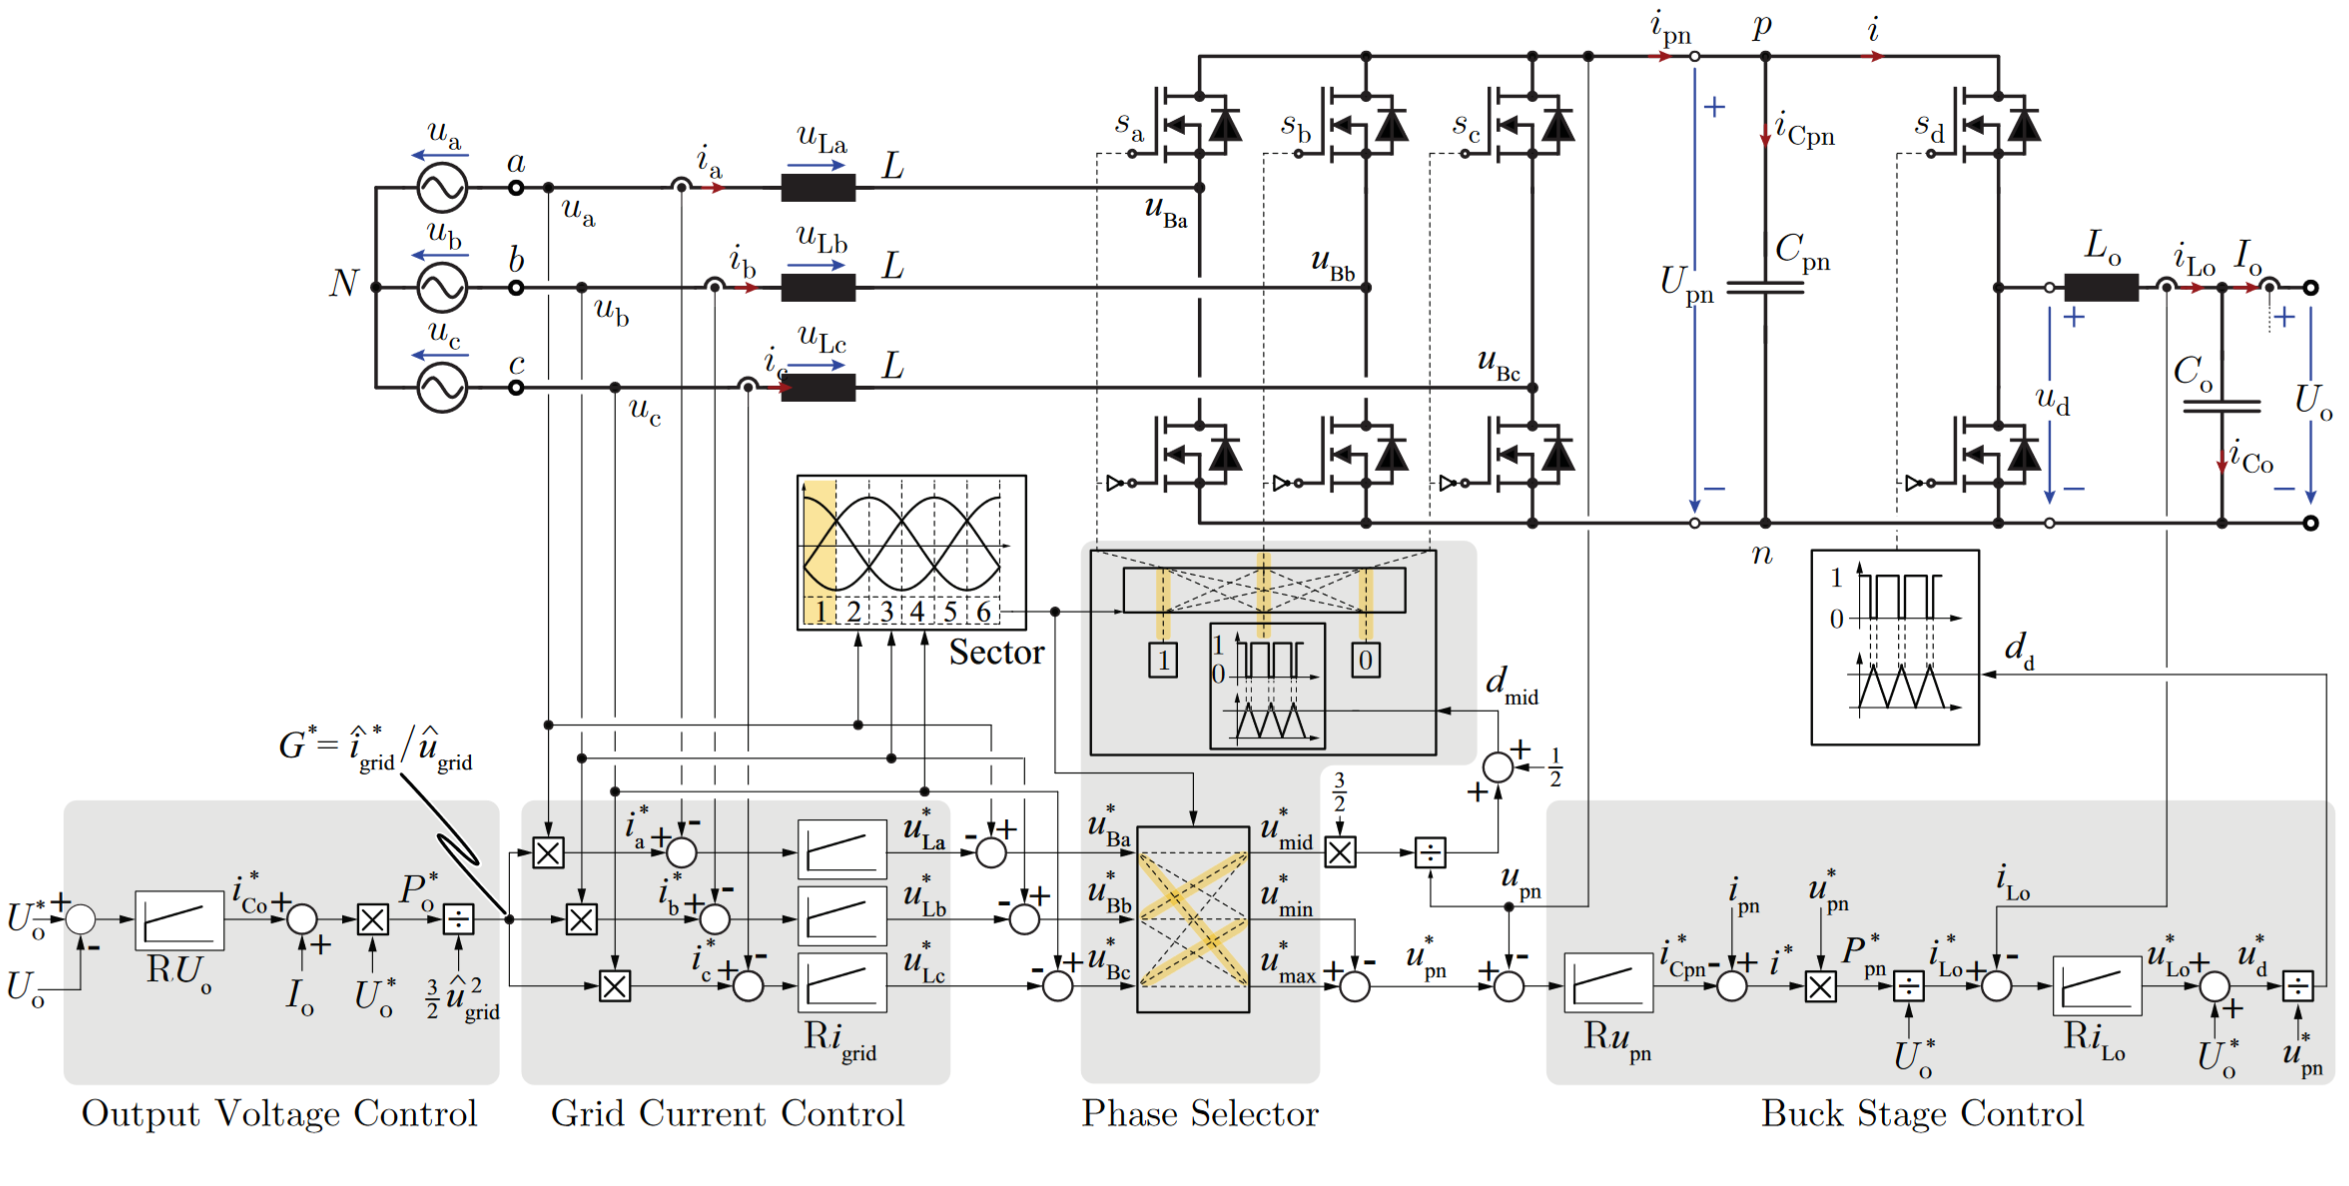
\includegraphics[width=0.9\linewidth]{content/Grafiken/B6-Control-orig}
	\caption[Regelung des \gls{B6PFC}]{Regelung des \gls{B6PFC} \cite{13PWMPFC}}
	\label{fig:b6-control-orig}
\end{figure}
